%\section{Automatic nested loop acceleration design framework} \label{sec:acc-framework}
\section{Nested Loop Accelerator Design Framework} \label{sec:acc-framework}
By using a regular SCGRA overlay built on top of the physical FPGA devices, 
we have developed an automatic nested loop acceleration framework called QuickDough.
QuickDough targets hybrid CPU-FPGA
computing systems where the FPGA is devoted to accelerating compute intensive loop kernel and CPU handles the
rest of the application.
%To that end, a standard software compilation routine is included to produce binary code for the CPU.
\figref{fig:framework} depicts an overview of the design framework, highlighting the complementary \emph{accelerator generation} and \emph{accelerator customization} paths.

By design, the steps along the accelerator generation path are short and essential during rapid design iterations.  Collectively, they are able to generate FPGA loop accelerators making use of a pre-built bitstream library in the order of seconds \cite{scgra}.

Meanwhile, the focus of this paper is on the accelerator customization path, which is relatively slow but is necessary for improving performance of the resulting accelerators on a per-application basis.
%
These steps automatically tunes the design parameters 
including overlay architectural parameters, compilation options as well as communication between the
FPGA accelerator and host processor specifically to a user application under user constraints
such as hardware resource budgets.
With the customized design 
parameters, HDL models of the corresponding SCGRA overlay and their associated drivers are then
generated. Afterwards, the drivers will be used by the software compiler while the FPGA
accelerator will be implemented and stored in the accelerator library, which can be reused by the
fast accelerator generation path in subsequent compilations.

\begin{figure}[tb]
\center{\includegraphics[width=0.85\linewidth]{framework}}
\caption{Automatic nested loop acceleration framework}
\label{fig:framework}
\vspace{-1.5em}
\end{figure}

\subsection{SCGRA based FPGA accelerator}
\figref{fig:scgra-acc} shows the design of a typical SCGRA overlay 
based FPGA accelerator. In the accelerator, on-chip
memory i.e. IBuf and OBuf are used to buffer the communication 
data between the host CPU and 
the accelerator. A controller is also presented in hardware 
to control the operations of the accelerator as well as
memory transfers. The SCGRA, which is the kernel computation fabric,
consists of an array of PEs and it achieves the computation 
task through the distributed control words stored in each PE. The AddrBuf 
stores all the valid IO buffer accessing addresses of the computation. 
The current implementation of a PE template is also presented in this figure. 
At the heart of the PE is an ALU, which is supported by a multi-port 
data memory and an instruction memory. Data memory stores intermediate data during the computation
while instruction memory stores all control words that determines the action of the PE. 
In addition, a global signal from the AccCtrl block controls the start/stop of all PEs in the array.

\begin{figure}[tb]
\center{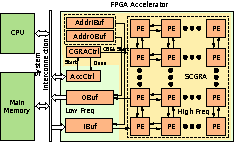
\includegraphics[width=0.7\linewidth]{scgra-accelerator}}
\caption{SCGRA overlay based FPGA accelerator}
\label{fig:scgra-acc}
\end{figure}

\subsection{Loop execution on the FPGA accelerator}
\figref{fig:group-dfg} illustrates how the loop is executed 
on the FPGA accelerator. First of all, 
data flow graph (DFG) is extracted from the loop and then it 
is scheduled on to the SCGRA overlay based FPGA accelerator. 
Depending on how much the loop is unrolled and transformed 
to DFG, the DFG may be executed repeatedly until the end of 
the original loop. In addition, data transfers for 
multiple executions of the same DFG are batched into groups 
as shown in \figref{fig:group-dfg}. On the one hand, this technique is used to 
reduce the number of batching, which further helps to amortize 
the initial communication cost. On the other hand, it also 
results in larger on-chip memory overhead. The proposed customization framework 
can be used to make the right design choices to achieve an optimal design. 

\begin{figure}[tb]
\center{\includegraphics[width=0.62\linewidth]{group-dfg}}
\caption{Loop, group and DFG. The loop will be divided into 
groups. Each group will be partially unrolled and the unrolled part will be 
translated to DFG. IO transmission between FPGA and host CPU is performed 
in the granularity of a group.}
\label{fig:group-dfg}
\vspace{-2em}
\end{figure}

\subsection{SCGRA overlay compilation}
With pre-built SCGRA overlay library and customized overlay configuration, the corresponding FPGA
accelerator can be generated rapidly, which is also the basis of the high-productivity loop
accelerator design framework. \figref{fig:detailed-compilation} presents the detailed SCGRA overlay compilation. 
With the specified loop unrolling and grouping factor, DFG is generated and scheduled to the SCGRA
overlay of the accelerator. After the scheduling, control words are extracted, and they can 
further be integrated into the pre-built FPGA accelerator bitstream creating 
the final FPGA loop accelerator bitstream. The compilation process typically completes in a few
seconds as illustrated in \cite{scgra} which is particularly important during early application
development phases. 

\begin{figure}[tb]
\center{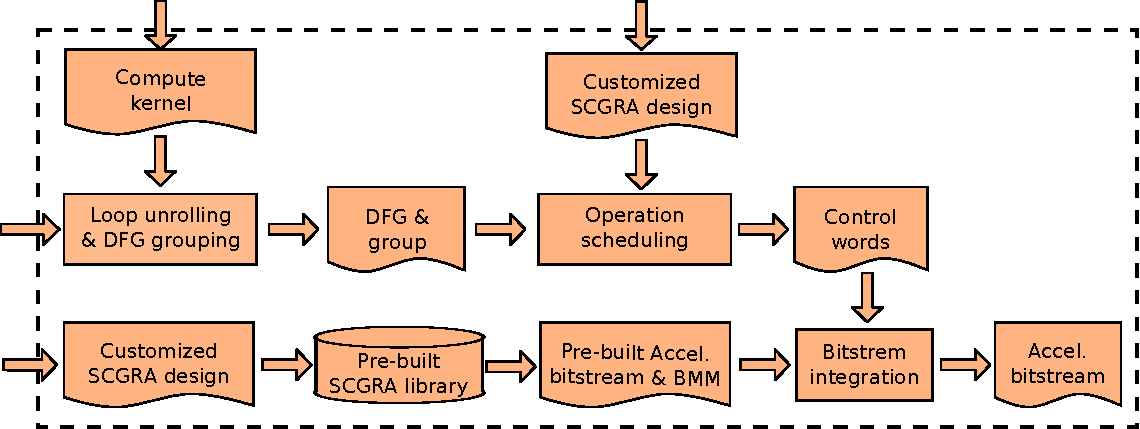
\includegraphics[width=0.95\linewidth]{detailed-compilation}}
\caption{Rapid SCGRA overlay compilation}
\label{fig:detailed-compilation}
\vspace{-1.5em}
\end{figure}



